\section[Conditional Random Fields]{Hidden Markov Models and Conditional Random Fields}

\Glspl{crf}\cite{originalCRF} are a graph-based modelling technique also used in sequence tagging commonly used in conjunction with \glspl{rnn} to improve classification accuracy. They can be understood as extensions to hidden Markov models.

\subsection{Hidden Markov Models}

    Hidden Markov models (HMMs) are based on markov processes. Markov processes describe a sequence of possible events in which the probability of each event depends \textit{only} on the state attained in the \textit{previous event}\cite{gagniuc2017markov}.
    HMMs consist of two such Markov processes: one process $\mathcal{X}$ with states that can be observed, such as a sequence of words, and one hidden process $\mathcal{Y}$ that depend on $\mathcal{X}$. The goal is to learn about $\mathcal{Y}$ by observing $\mathcal{X}$. HMMs use Bayesian modelling and apply them to Markov processes to make predictions\cite{klinger2007classical}.
   
   %TODO: Fix notation of $X, Y$ 
    \begin{figure}[t]
        \centering
        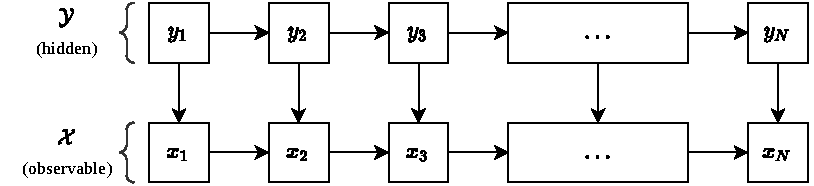
\includegraphics[width=0.90\textwidth]{hmm.pdf}
        \caption{In HMMs and CRFs, a hidden sequence $\mathcal{Y}$ is classified based on an an observable sequence $\mathcal{X}$.}
        \label{fig: HMM and CRF}
    \end{figure}

\subsection{Conditional Random Fields}
    \Glspl{crf} are a generalisation of HMM's that make fewer assumptions about probability distributions. Specifically, no assumptions on the dependencies among $x_{i} \in \mathcal{X}$ are made\cite{klinger2007classical}. Similar to how HMMs are Bayesian modelling applied to Markov processes, \glspl{crf} are an application of maximum entropy modelling to sequences\cite{klinger2007classical}.